O modelo solicitado para integração via requisição do tipo \textit{GET} no endpoint \textit{“/orders/opened”} na API do software principal do estabelecimento é exemplificado na \autoref{fig:drPlacedAPI}. O retorno da consulta deve ser em formato JSON, dispostos no formato “chave”: “valor” e contendo os seguinte atributos documentados pelo administrador: \textit{id}, \textit{latitude}, \textit{longitude}, \textit{payment\_id}, \textit{totalPrice}, \textit{prepaid} e \textit{status}.

\begin{figure}[H]
    \centering
    \caption{Delivery Routes - API - Coleta de dados}
    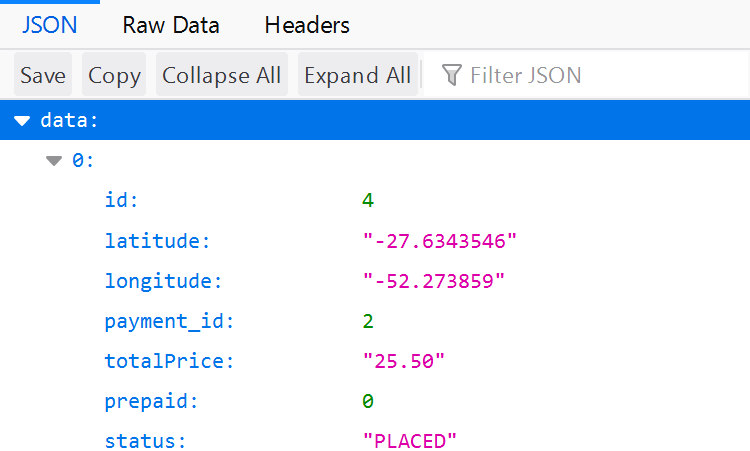
\includegraphics[width=0.6\textwidth]{./dados/figuras/fig14}
    \fonte{Autor}
    \label{fig:drPlacedAPI}
\end{figure}